%%%%%%%%%%%%%%%%%%%%%%%%%%%%%%%%%%%%%%%%%
% Masters/Doctoral Thesis 
% LaTeX Template
% Version 2.5 (27/8/17)
%
% This template was downloaded from:
% http://www.LaTeXTemplates.com
%
% Version 2.x major modifications by:
% Vel (vel@latextemplates.com)
%
% This template is based on a template by:
% Steve Gunn (http://users.ecs.soton.ac.uk/srg/softwaretools/document/templates/)
% Sunil Patel (http://www.sunilpatel.co.uk/thesis-template/)
%
% Template license:
% CC BY-NC-SA 3.0 (http://creativecommons.org/licenses/by-nc-sa/3.0/)
%
%%%%%%%%%%%%%%%%%%%%%%%%%%%%%%%%%%%%%%%%%

%----------------------------------------------------------------------------------------
%	PACKAGES AND OTHER DOCUMENT CONFIGURATIONS
%----------------------------------------------------------------------------------------

%\input{Sections/Packages}
%----------------------------------------------------------------------------------------
%	PACKAGES AND OTHER DOCUMENT CONFIGURATIONS
%----------------------------------------------------------------------------------------

\documentclass[
11pt, % The default document font size, options: 10pt, 11pt, 12pt
oneside, % Two side (alternating margins) for binding by default, uncomment to switch to one side
english, % ngerman for German
singlespacing, % Single line spacing, alternatives: onehalfspacing or doublespacing
%draft, % Uncomment to enable draft mode (no pictures, no links, overfull hboxes indicated)
%nolistspacing, % If the document is onehalfspacing or doublespacing, uncomment this to set spacing in lists to single
%liststotoc, % Uncomment to add the list of figures/tables/etc to the table of contents
%toctotoc, % Uncomment to add the main table of contents to the table of contents
parskip, % Uncomment to add space between paragraphs
%nohyperref, % Uncomment to not load the hyperref package
headsepline, % Uncomment to get a line under the header
%chapterinoneline, % Uncomment to place the chapter title next to the number on one line
%consistentlayout, % Uncomment to change the layout of the declaration, abstract and acknowledgements pages to match the default layout
]{MastersDoctoralThesis} % The class file specifying the document structure
\usepackage{listings}
\usepackage{xcolor}
\usepackage{float}
\usepackage{caption}
\usepackage{subcaption}
\usepackage{datetime}
\usepackage[final]{hyperref}
\usepackage{comment}
\usepackage{microtype}
\usepackage{booktabs} % For better table lines
\usepackage{tabularx} % For adjustable-width columns
\usepackage{ltablex} % Combines tabularx and longtable
\usepackage{pdflscape} % For landscape pages
\usepackage{tikz} % For drawing figures
\usepackage{adjustbox} % For resizing tables
\usepackage{graphicx}
\usepackage{pgfplots}
\usetikzlibrary{shapes.geometric, arrows.meta, decorations.pathreplacing,positioning,fit,backgrounds, calc} % For relative positioning of nodes
\newdateformat{monthyeardate}{\monthname[\THEMONTH] \THEYEAR}

\definecolor{codegreen}{rgb}{0,0.6,0}
\definecolor{codegray}{rgb}{0.5,0.5,0.5}
\definecolor{codepurple}{rgb}{0.58,0,0.82}
\definecolor{backcolour}{rgb}{0.95,0.95,0.92}
\definecolor{yellow25}{RGB}{255, 230, 153}
\definecolor{orange25}{RGB}{255, 229, 191} % Light orange
\definecolor{green25}{RGB}{191, 255, 191} % Light green
\definecolor{blue25}{RGB}{191, 229, 255} % Light blue
\definecolor{purple25}{RGB}{229, 191, 255} % Light purple
\definecolor{red25}{RGB}{255, 204, 204}

\lstdefinestyle{mystyle}{
    backgroundcolor=\color{backcolour},   
    commentstyle=\color{codegreen},
    keywordstyle=\color{magenta},
    numberstyle=\tiny\color{codegray},
    stringstyle=\color{codepurple},
    basicstyle=\ttfamily\footnotesize,
    breakatwhitespace=faòse,         
    breaklines=true,                 
    captionpos=b,                    
    keepspaces=true,                 
    numbers=left,                    
    numbersep=5pt,                  
    showspaces=false,                
    showstringspaces=false,
    showtabs=false,                  
    tabsize=2
}

\lstset{style=mystyle}

\usepackage[utf8]{inputenc} % Required for inputting international characters
\usepackage[T1]{fontenc} % Output font encoding for international characters

\usepackage{mathpazo} % Use the Palatino font by default
\usepackage{amsmath}
\usepackage{bbm}

\usepackage[
backend=biber,
style=numeric,
sorting=nty
]{biblatex}

\addbibresource{sample.bib} % The filename of the bibliography

\usepackage[autostyle=true]{csquotes} % Required to generate language-dependent quotes in the bibliography

%----------------------------------------------------------------------------------------
%	MARGIN SETTINGS
%----------------------------------------------------------------------------------------

\geometry{
	paper=a4paper, % Change to letterpaper for US letter
	inner=2.5cm, % Inner margin
	outer=3.8cm, % Outer margin
	bindingoffset=.5cm, % Binding offset
	top=1.5cm, % Top margin
	bottom=1.5cm, % Bottom margin
	%showframe, % Uncomment to show how the type block is set on the page
}
\pgfplotsset{compat=1.16}
\tikzset{
  state/.style={circle, draw, minimum size=1.5cm}, % Define the state style
  observation/.style={circle, draw, fill=gray!10, minimum size=1cm}, % Define the observation style
  gate/.style={draw,rectangle,fill=yellow!20,minimum size=10mm},
  operator/.style={draw,circle,fill=red!30,minimum size=5mm},
  point/.style={coordinate},
  layer/.style={draw,thick,dashed,rectangle,minimum height=30mm,minimum width=10mm,fill=blue!10},
  path/.style={->,>=stealth,thick},
  label/.style={text centered}
}

%----------------------------------------------------------------------------------------
%	THESIS INFORMATION
%----------------------------------------------------------------------------------------

%----------------------------------------------------------------------------------------
%	THESIS INFORMATION
%----------------------------------------------------------------------------------------

\thesistitle{Predictive algorithm and guidance for human motion in robotics teleoperation} % Your thesis title, this is used in the title and abstract, print it elsewhere with \ttitle
\supervisor{Alessandro  \textsc{Rizzo} \\(\textit{Politecnico di Torino})} % Your supervisor's name, this is used in the title page, print it elsewhere with \supname
\cosupervisor{Domenico \textsc{Prattichizzo} \\(\textit{Università di Siena})} % Your co-supervisor's name, this is used in the title page, print it elsewhere with \cosupname
\cocosupervisor{Enrico \textsc{Turco} \\(\textit{Istituto Italinao di Tecnologia})} % Your co-supervisor's name, this is used in the title page, print it elsewhere with \cosupname
\cococosupervisor{Valerio \textsc{Bo} \\(\textit{Istituto Italinao di Tecnologia})} % Your co-supervisor's name, this is used in the title page, print it elsewhere with \cosupname

\examiner{} % Your examiner's name, this is not currently used anywhere in the template, print it elsewhere with \examname
\degree{} % Your degree name, this is used in the title page and abstract, print it elsewhere with \degreename
\author{Francesco \textsc{Stolcis}} % Your name, this is used in the title page and abstract, print it elsewhere with \authorname
\addresses{} % Your address, this is not currently used anywhere in the template, print it elsewhere with \addressname

\subject{Mechatronic Engineering} % Your subject area, this is not currently used anywhere in the template, print it elsewhere with \subjectname
\keywords{} % Keywords for your thesis, this is not currently used anywhere in the template, print it elsewhere with \keywordnames
\university{Politecnico di Torino} % Your university's name and URL, this is used in the title page and abstract, print it elsewhere with \univname
\department{Department or Control and Computer Engineering} % Your department's name and URL, this is used in the title page and abstract, print it elsewhere with \deptname
\group{\href{http://researchgroup.university.com}{}} % Your research group's name and URL, this is used in the title page, print it elsewhere with \groupname
\faculty{Mechatronic Engineering} % Your faculty's name and URL, this is used in the title page and abstract, print it elsewhere with \facname

\AtBeginDocument{
\hypersetup{pdftitle=\ttitle} % Set the PDF's title to your title
\hypersetup{pdfauthor=\authorname} % Set the PDF's author to your name
\hypersetup{pdfkeywords=\keywordnames} % Set the PDF's keywords to your keywords
}

%----------------------------------------------------------------------------------------
%	BEGIN DOCUMENT
%----------------------------------------------------------------------------------------

\begin{document}

\frontmatter % Use roman page numbering style (i, ii, iii, iv...) for the pre-content pages

\pagestyle{plain} % Default to the plain heading style until the thesis style is called for the body content

%----------------------------------------------------------------------------------------
%	TITLE PAGE
%----------------------------------------------------------------------------------------

\include{Sections/Title}

%----------------------------------------------------------------------------------------
%	DECLARATION PAGE
%----------------------------------------------------------------------------------------

%\include{Sections/Declaration}

%----------------------------------------------------------------------------------------
%	QUOTATION PAGE
%----------------------------------------------------------------------------------------

%\include{Sections/Quotation}

%----------------------------------------------------------------------------------------
%	ABSTRACT PAGE
%----------------------------------------------------------------------------------------

%----------------------------------------------------------------------------------------
%	ABSTRACT PAGE
%----------------------------------------------------------------------------------------

\begin{abstract}
\addchaptertocentry{\abstractname} % Add the abstract to the table of contents
This thesis proposes a novel approach for enhancing the teleoperation of robotic arms through shared control mechanisms, integrating advanced machine learning techniques and classical control methods. The primary objective is to develop a robust system capable of autonomously guiding the robotic arm towards predicted objects while maintaining operator oversight. The framework employs a Long Short-Term Memory (LSTM) classification model to predict the location and nature of objects within the robot's workspace. This predictive capability enables the system to anticipate the operator's intentions and adaptively plan trajectories. Furthermore, artificial potential fields are utilized to generate guidance commands that assist the operator in maneuvering the robotic arm towards the predicted objects. By combining the predictive power of LSTM with the reactive nature of potential fields, the system achieves a seamless fusion of human expertise and autonomous control, ensuring both efficiency and safety in teleoperation tasks. The proposed approach is implemented and validated through comprehensive simulations and real-world experiments using a teleoperated robotic arm platform. Performance evaluations demonstrate the effectiveness and reliability of the shared control system, showcasing improved object manipulation capabilities and reduced cognitive workload for the operator. Additionally, the system's adaptability to varying environmental conditions and object dynamics is examined, highlighting its potential for deployment in diverse teleoperation scenarios. Overall, this thesis contributes to the advancement of teleoperated robotic systems by introducing a novel framework that seamlessly integrates machine learning and classical control techniques. The proposed shared control approach offers enhanced capabilities for object manipulation tasks, paving the way for more efficient and intuitive human-robot collaboration in various domains, including manufacturing, healthcare, and disaster response.
\end{abstract}

%----------------------------------------------------------------------------------------
%	LIST OF CONTENTS/FIGURES/TABLES PAGES
%----------------------------------------------------------------------------------------

\include{Sections/Lists}

%----------------------------------------------------------------------------------------
%	DEDICATION
%----------------------------------------------------------------------------------------

%\dedicatory{For/Dedicated to/To my\ldots} 

%----------------------------------------------------------------------------------------
%	THESIS CONTENT - CHAPTERS
%----------------------------------------------------------------------------------------

\mainmatter % Begin numeric (1,2,3...) page numbering

\pagestyle{thesis} % Return the page headers back to the "thesis" style

% Include the chapters of the thesis as separate files from the Chapters folder
% Uncomment the lines as you write the chapters

\include{Chapters/Chapter1}



% Chapter Template

\chapter{State of the Art} % Main chapter title

\label{Chapter2} % Change X to a consecutive number; for referencing this chapter elsewhere, use \ref{ChapterX}

%----------------------------------------------------------------------------------------
%	SECTION 1
%----------------------------------------------------------------------------------------
This thesis project focuses on the concept of shared control during the teleoperation of a robotic arm.
In this context it is important to define firstly the concept of teleoperation and the architecture of a telerobotic system, subsequently the shared control case.
\section{Teleoperation}
\subsection{Teleoperation system }
Teleoperation, a field at the intersection of robotics, control systems, and telecommunications, represents a advacement of the human action in scenarios where direct human involvement is impractical, hazardous, or impossible. 
At its core, teleoperation involves the remote control of machines, robots, or other systems, where the operator is at a significant distance from the equipment being controlled. This separation can range from a few meters, as in bomb disposal robots, to thousands of kilometers, as seen in space rovers operated from Earth.

The operational framework of teleoperation systems is rappresented by several key components: 
\begin{itemize}
    \item\textbf{the operator control unit (OCU):} The OCU serves as the interface through which the human operator interacts with the teleoperation system, typically featuring control devices like joysticks, gloves, or even more sophisticated haptic devices that provide tactile feedback, simulating the sensation of touch. This feedback is crucial, as it enhances the operator's ability to perform complex manipulations remotely by offering a semblance of physical presence at the teleoperator's location.
    
    \item\textbf{the teleoperator :} The teleoperator, equipped with various sensors, actuators, and sometimes autonomous control capabilities, executes the tasks directed by the operator. These tasks can range from simple pick-and-place operations to intricate surgical procedures, depending on the system’s design and intended application. The sophistication of the teleoperator is a critical factor in the system’s overall performance, particularly its ability to execute precise movements and provide feedback that accurately reflects the remote environment.
    
    \item\textbf{communication link:} Bridging the OCU and the teleoperator is the communication link, which can be wired or wireless, depending on the application's requirements and constraints. This link transmits control signals from the operator to the teleoperator and sends sensory feedback (visual, haptic, etc.) back to the operator. The quality of this link, in terms of latency, bandwidth, and reliability, significantly impacts the system's effectiveness and the operator's ability to control the teleoperator accurately and responsively.

\end{itemize}

An overview of a telerobotic system can be expressed as follow:
\begin{figure}[th]
    \centering
    \includegraphics[scale=0.6]{Figures/Chapter2/teleoperation.png}
    \caption[telerobotic system]{telerobotic system}
    \label{fig:telerobotic system}
\end{figure}


\subsection{Telerobotic Architecture}
The architecture of a telerobotic system is a critical factor in determining the effectiveness, safety, and usability of the system. The architecture defines the interaction between the human operator and the teleoperator, the distribution of control tasks, and the level of autonomy in the system. The choice of architecture depends on the specific task requirements, the complexity of the environment, the operator's expertise, and the capabilities of the teleoperator.
There are three architectures structures for telerobotic systems, each with distinct characteristics and applications:
\begin{itemize}
    \item\textbf{Direct Control:} Direct Control is the simplest form of teleoperation, where every action taken by the human operator is directly translated into movements or actions of the teleoperator. This one-to-one correspondence means that the operator has immediate and complete control over the teleoperator's actions. Direct control systems are highly dependent on the operator's skill and attention, as there is minimal to no automation involved. This architecture is most effective in environments where precise, real-time control is necessary, and the task complexity is manageable by the human operator without additional automated support.

    \item\textbf{Shared Control:} Shared Control represents a more advanced teleoperation approach, where control is divided between the human operator and autonomous system functions. In this architecture, the operator and the teleoperation system share the task of controlling the teleoperator. The distribution of control can be dynamic, with the level of automation adjusting based on the task complexity, operator workload, or other contextual factors. Shared control systems are designed to combine human cognitive abilities with the precision and reliability of automated systems, optimizing task performance and potentially reducing operator fatigue. This approach is particularly beneficial in complex or unpredictable environments, where human judgment is essential, but so is the efficiency and consistency of automated processes.

    \item\textbf{Supervisory Control:} Supervisory Control takes a step further in integrating automation into teleoperation. In this architecture, the human operator takes on a supervisory role, monitoring the operation and intervening only when necessary. The teleoperator, equipped with a higher degree of autonomy, can perform tasks independently based on pre-programmed instructions or algorithms. The operator's primary responsibilities include setting goals, specifying constraints, monitoring progress, and intervening in case of unexpected events or system failures. Supervisory control is well-suited for operations in highly dangerous or inaccessible environments, or for tasks that require extended periods, where continuous direct human control is impractical.

\end{itemize}

%----------------------------------------------------------------------------------------
%	SECTION 2
%----------------------------------------------------------------------------------------

\section{Shared Control}
\label{Chapter2/PerspProj}
The adopted architectur to infer the teleoperation of the robotic arm is the shared control one, aiming to combine human cognitive capabilities with robotic efficiency to reduce the operator's workload and enhance task performance.\\
This architecture is pivotal in scenarios where fully autonomous robotic control is unfeasible due to unpredictable and complex environments.\\ 
More specifically, there are three main ways to implement the shared control architectur: Semi-Autonomous Control (SAC), State-Guidance Shared Control (SGSC), and State-Fusion Shared Control (SFSC).

\begin{itemize}
    \item\textbf{Semi-Autonomous Control (SAC):}In SAC the division of control tasks between the human operator and the autonomous system is distinctly demarcated. In this approach, the autonomous system and the human operator control separate variables, allowing each to leverage their strengths for improved task execution. This delineation enables the human operator to focus on high-level decision-making and strategic task elements, while the autonomous system manages the execution of routine or precise actions.\\ 
    The SAC model is particularly beneficial in complex and dynamic environments where human intuition and strategic oversight are crucial for success but are complemented by the precision and reliability of autonomous robotic actions. It facilitates a collaborative interaction where the operator's cognitive load is reduced, and the efficiency and safety of operations are enhanced by offloading specific control tasks to the robotic system

    \item\textbf{State-Guidance Shared Control (SGSC):} In SGSC the autonomous system provides direct guidance to the human operator, which can take various forms such as visual, auditory, or haptic feedback. This guidance is designed to assist the operator in making more informed decisions or in executing tasks with greater precision.\\ 
    The key principle behind SGSC is to enhance the operator's situational awareness and to facilitate the decision-making process without overtaking the human's control. This is achieved by allowing the autonomous system to suggest or warn the operator based on the system's perception and analysis of the environment or the task at hand. SGSC strategies are particularly useful in scenarios where human intuition and judgment are critical, but where the complexity or danger of the task necessitates additional inputs that can augment human capabilities. By providing guidance, SGSC aims to reduce the cognitive load on the operator, improve task performance, and enhance safety without diminishing the human's role in the control loop

    \item\textbf{State-Fusion Shared Control (SFSC):} SFSC  strategy goes beyond merely dividing tasks or providing guidance; it integrates the intentions and control signals of the human operator and the robot through a fusion mechanism. The fusion process often involves sophisticated algorithms that can weigh the contributions of the human and the robot based on factors like task complexity, operator expertise, and system capabilities. \\
    The goal of SFSC is to harness the strengths of both human and machine: the adaptability, judgment, and intuition of the human, alongside the precision, reliability, and speed of the machine. This integrated approach allows for a more seamless and efficient execution of tasks, particularly in environments that are too complex for fully autonomous robotics or require a level of decision-making beyond current autonomous capabilities. By dynamically adjusting the level of influence between human and machine based on real-time feedback and task requirements, SFSC strategies ensure that the control system remains adaptable and responsive to the nuances of each specific operation. This not only improves the performance and safety of telerobotic systems but also enhances the user experience by creating a more intuitive interaction between the human operators and the robotic system.

\end{itemize}
\begin{figure}[ht]
    \centering
    \begin{subfigure}[a]{0.32\textwidth}
      \includegraphics[width=\textwidth]{Figures/Chapter2/shared_1.png}
      \caption{Semi-Autonomous Control}
      \label{fig:semi_auto_control}
    \end{subfigure}
    \hfill % This will add horizontal space between the figures
    \begin{subfigure}[b]{0.32\textwidth}
      \includegraphics[width=\textwidth]{Figures/Chapter2/shared_2.png}
      \caption{Cooperative Control}
      \label{fig:cooperative_control}
    \end{subfigure}
    \hfill % This will add horizontal space between the figures
    \begin{subfigure}[c]{0.32\textwidth}
      \includegraphics[width=\textwidth]{Figures/Chapter2/shared_3.png}
      \caption{Supervised Autonomous Control}
      \label{fig:supervised_auto_control}
    \end{subfigure}
    \caption{Types of Shared Control}
    \label{fig:shared_control_types}
  \end{figure}
  
In the context of this project the share controll architecture is implemented through the SFSC strategy. Since the aim is to help the teleoperator during teleoperation, this strategy ensures that the human operator and the robotic system can work together seamlessly, leaving the operator in control of the task while providing the necessary support and assistance to enhance task performance and safety.\\
To properly implement the strategy, the problem has to suibdivided into three main compartements: intention recognition, guidance and autonomous control.





%----------------------------------------------------------------------------------------
%	SECTION 3
%----------------------------------------------------------------------------------------\\     
\section{Intention Recognition}
The core challenge of intention recognition lies in accurately inferring the user's goals from a set of possible actions, often in real-time and under uncertainty. This process involves the collection and analysis of data generated by human actions, which could be in the form of physical movements, verbal commands, or control signals. The ultimate aim is to enable robots or autonomous systems to anticipate the needs or next actions of their human partners, allowing for proactive assistance.

\subsection{Metodologies}

Intention recognition methodologies span a range of approaches, reflecting the diversity of applications and the complexity of interpreting human intent.\\
At this day, there isn't a single, universally accepted method for intention recognition that applies across all scenarios in the teleoperation of robotic arms. Instead, the field comprises a variety of techniques, each with its strengths and limitations, tailored to specific contexts, tasks, and environments
\begin{itemize}
    \item\textbf{Probabilistic Models:} Techniques such as Hidden Markov Models (HMMs), as extensively explained in \cite{5480475} and \cite{AARNO2008692},is a statistical model that represents systems with probabilistic properties.
    It is characterized by its ability to model systems where the states are hidden and not directly observable, but the outcomes or observations associated with these states are observable.\\
    An HMM is defined by three primary elements: the state transition probability matrix $\textbf{A}$, which specifies the likelihood of transitioning from one state to another; the observation probability matrix $\textbf{B}$, detailing the probability of observing a certain symbol when in a specific state; and the initial state probability vector $\boldsymbol{\pi}$, indicating the likelihood of the system starting in each state.\\
    
    % Inserted TikZ Picture

    

    
    \begin{figure}[ht]
    \centering
    \begin{adjustbox}{center} 
    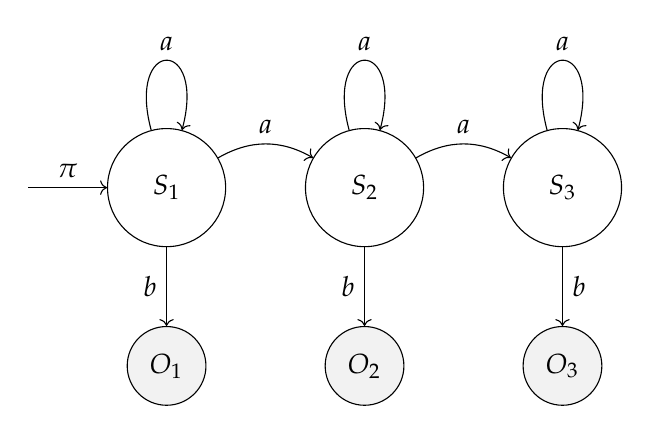
\begin{tikzpicture}
       
        % States
        \node[state] (s1) {$S_1$};
        \node[state] (s2) [right=of s1] {$S_2$};
        \node[state] (s3) [right=of s2] {$S_3$};
    
        % Observations
        \node[observation] (o1) [below=of s1] {$O_1$};
        \node[observation] (o2) [below=of s2] {$O_2$};
        \node[observation] (o3) [below=of s3] {$O_3$};
    
        % State transitions
        \draw[->] (s1) to[bend left] node[midway,above] {$a$} (s2);
        \draw[->] (s2) to[bend left] node[midway,above] {$a$} (s3);
        \draw[->] (s1) to[loop above] node[midway,above] {$a$} (s1);
        \draw[->] (s2) to[loop above] node[midway,above] {$a$} (s2);
        \draw[->] (s3) to[loop above] node[midway,above] {$a$} (s3);
    
        % Observations
        \draw[->] (s1) -- (o1) node[midway,left] {$b$};
        \draw[->] (s2) -- (o2) node[midway,left] {$b$};
        \draw[->] (s3) -- (o3) node[midway,right] {$b$};
    
        % Initial state probabilities
        \draw[->] ([xshift=-1cm]s1.west) -- (s1) node[midway,above] {$\pi$};
    \end{tikzpicture}
    \end{adjustbox}
    \hspace{5mm}
    \begin{adjustbox}{valign=t}
        % Legend
    \begin{minipage}[b]{0.4\textwidth}
            %\flushright % Adjusts the alignment of the legend to the right
            \textbf{Legend:}\\
            S: State\\
            O: Observation\\
            $a$: Transition Probability\\
            $b$: Observation Probability\\
            $\pi$: Initial State Probability
    \end{minipage}
    \end{adjustbox}
    \label{fig:Representation of a Hidden Markov Model (HMM)}
    \caption{Representation of a Hidden Markov Model (HMM)}
    \end{figure}
    
    As outlined in , while the application of HMMs in intention recognition for teleoperated robotic arm manipulation offers notable advantages in handling temporal dynamics and model flexibility, it concurrently presents substantial challenges, particularly in the necessity for precise and well-documented a priori knowledge.
    The complex nature of human decision-making processes complicates the task of accurately predicting operator behavior at each timestep of the teleoperation task; this is evident in the methodology, where the transition matrix $\textbf{A}$ is constructed based on empirical observations. This approach results in a relatively simplistic policy for state transitions, potentially oversimplifying the nuanced and variable nature of human intent during teleoperation tasks.
    





    \item\textbf{Inverse Reinforcement Learning (IRL):} Inverse Reinforcement Learning (IRL) is a sophisticated method for deciphering and forecasting the intentions behind human operators' actions in teleoperation, where understanding complex decision-making is key to enhancing human-robot interactions.\\
    Brian D. Ziebart et al.~\cite{ziebart2008maximum} extend IRL's capabilities through a probabilistic framework grounded in the maximum entropy principle, adept at navigating the uncertainties in teleoperation decision-making. 
    This approach, by favoring the least biased action distribution based on observed behaviors, provides a refined representation of operators' reward functions, thus accurately modeling their intent.\\
    The incorporation of maximum entropy IRL into intent recognition significantly improves how robotic systems can preemptively adjust to and fulfill human operator goals, shifting from merely reactive to proactive adaptations.
    Despite these advancements, implementing IRL in real-time applications is hindered by the extensive computational resources needed to process complex data and infer human intent in a fast and accurate manner, presenting a challenge in the practical deployment of IRL-enhanced robotic systems.
    
    \item\textbf{Partially Observable Markov Decision Processes (POMDPs):} Partially Observable Markov Decision Processes (POMDPs) are a class of decision-making models that consider situations where the state of the system is partially observable or uncertain to the decision-maker. 
    In a POMDP framework, the decision-maker must rely on observations that may provide indirect or incomplete information about the system's state to make decisions. 
    This model extends the Markov Decision Process (MDP) framework by incorporating a layer of uncertainty regarding the system's actual state, making it particularly suited for complex environments where full information is not available.\\
    In the context of shared control systems, POMDPs play a crucial role in modeling the interaction between a human user and an autonomous system, especially when the system's understanding of the user's intent is uncertain.
    the authors in \cite{doi:10.1177/0278364918776060} delve into this by formalizing shared autonomy as a POMDP, which assists in minimizing the expected cost-to-go with an unknown goal.
    This approach acknowledges that while the autonomous system may not confidently predict the user's specific goal until it is nearly achieved, it can still offer valuable assistance by optimizing actions that are generally helpful across multiple potential goals.
    When the system has high confidence in a single user goal, the framework focuses assistance more narrowly to support that specific objective. This balance allows for more effective and adaptive assistance, even in the face of uncertainty about the user's exact intentions.\\
    Despite its great ability to handle uncertainty, give focused help based on goals, and use hindsight optimization to make real-time processing better, this method still encounters problems with how complex its computations are, requiring substantial computational resources to function effectively.
    Additionally, the performance of this approach is deeply interconnected with the precision of its observational models for accurately perceiving and interpreting actions. 
    Inaccurate models significantly impair the system's capability to discern the user's intentions, leading to challenges in providing timely and relevant assistance. 
    Therefore, it is crucial to enhance the accuracy of these models to ensure they accurately reflect real-world scenarios, thereby optimizing the method's efficiency

    \item\textbf{Recurrent neural networks:} Recurrent Neural Networks (RNNs) are a specialized type of artificial neural networks crafted to recognize and interpret patterns in sequential data, including but not limited to text, genomic sequences, handwriting, or numerical time series from various sensors. What sets RNNs apart from traditional feedforward neural networks is their unique architecture featuring directed cycles in their connections.
    This design allows them to retain information over time, enabling the network to maintain a form of 'memory'.
    Such a capability is invaluable for tasks where understanding the context or the sequence in which data points appear is crucial.
    By iterating through elements in a sequence and maintaining a state that accumulates information seen thus far, RNNs effectively process sequences by leveraging their internal state (memory) to manage a range of inputs sequentially. This characteristic renders them incredibly useful for a variety of applications, including language modeling, speech recognition, and forecasting in time series data.
    Despite their advantages, RNNs are not without their challenges. Notably, they can be difficult to train effectively due to issues like vanishing and exploding gradients, which hinder their ability to learn long-range dependencies within the data.\\
    As elaborated in \cite{10.1162/neco_a_01199} to overcome these obstacles, Long Short-Term Memory (LSTM) networks emerge as a powerful solution within the domain of shared control of robotic arms, especially for tasks like intention prediction. 
    The LSTM, with its unique ability to learn and remember over long periods, has significantly improved the predictability and accuracy of user intention in shared control systems. This advanced form of RNN addresses the core limitations of its predecessors by efficiently handling long-term dependencies. 
    The robustness of Long Short-Term Memory (LSTM) networks against time gaps in data input, coupled with their capacity to adapt to individual user preferences, significantly boosts the efficiency and personalization of shared control systems.
    However, the sophisticated nature of LSTMs brings about challenges, including increased computational complexity and a greater need for extensive training data. Despite these challenges, the integration of LSTMs into Recurrent Neural Network (RNN) technology marks a significant leap forward. 
    It expands the potential for more intuitive and adaptable human-robot collaboration within shared control environments, navigating through the practical difficulties associated with their implementation.
\end{itemize}



%----------------------------------------------------------------------------------------
%	SECTION 4
%----------------------------------------------------------------------------------------
\section{Guidance}
In the domaine of shared control systems, guidance embodies a sophisticated integration of feedback and control strategies, facilitating seamless and intuitive interactions between humans and robots.
At the heart of guidance lies the objective to harmonize the decision-making capabilities and adaptability of human operators with the accuracy, reliability, and operational efficiency of robotic systems. 
This harmony is achieved through a continuous exchange of information, where the system furnishes the human operator with immediate, pertinent data, feedback, and actionable advice. 
This enables the operator to make well-informed decisions that guide the robot's actions. Such a reciprocal flow of information significantly enhances the effectiveness of task performance, elevates safety standards, and guarantees an advanced level of control and adaptability.
This acts as a critical link between human operators and automated systems, effectively reducing the workload.%-----------------------------------
%	SUBSECTION 1
%-----------------------------------
\subsection{Metodologies}

Guidance methodologies in shared control systems showcase a broad spectrum of approaches, highlighting the complex interplay between human operators and robotic mechanisms, especially in teleoperation scenarios;among these, Artificial Potential Fields (APF), the Dynamic Window Approach (DWA), the Vector Field Histogram (VFH), and Rapidly-exploring Random Trees (RRT) have been proven to be particularly effective in guiding robotic systems in shared control environments.\\

\begin{itemize}
    \item\textbf{Artificial Potential Fields (APF):} 
    The implementation of Artificial Potential Fields (APF) \cite{100007} is integral to enhancing real-time shared control in teleoperation frameworks, focusing on obstacle avoidance and efficient path planning. 
    APF employs virtual forces that guide the robotic system by creating a potential field where obstacles generate repulsive forces, and the goal exerts an attractive force. This dynamic allows the robot to navigate by following the gradient of the potential function, akin to traversing a landscape of peaks and valleys designed to steer clear of obstacles while being drawn toward the target.
    Upon setting a goal, APF aligns the robot's movement with the operator's intent by modulating these virtual forces, thereby facilitating an intuitive interaction between the human operator and the robotic system.\\
    The primary challenges associated with APF include the robot's susceptibility to getting trapped in local minima—regions where the potential gradient is zero, preventing further movement towards the goal—and the method's purely reactive nature to collision avoidance. 
    In standard APF applications, the robot alters its course only when in close proximity to obstacles, which may not be efficient for advanced navigation and obstacle avoidance in cluttered environments. 

    However, as presented in \cite{9734752}, the problem of obstacle avoidance in cluttered environments can be efficiently overcome with the dynamic generation of escape points around obstacles. 
    These escape points are designed to help the robotic system bypass obstacles smoothly while avoiding the pitfalls of local minima.\\ 
    This approach not only addresses the issue of the robot getting stuck but also allows for more proactive obstacle avoidance by modifying the robot's trajectory in advance, rather than merely reacting when close to obstacles.

    \item\textbf{Dynamic Window Approach (DWA):} he Dynamic Window Approach (DWA) is a fundamental technique in mobile robotics, utilized for motion planning and obstacle avoidance in dynamic environments. 
    It operates by constraining the robot's velocity to a "dynamic window," considering its current state and capabilities. 
    Within this window, potential velocities are evaluated using a cost function that incorporates factors such as obstacle distance, goal direction, and robot velocity. 
    By selecting the velocity that maximizes this function while ensuring collision-free navigation, the DWA facilitates rapid decision-making in real-time motion control.\\ 
    To fit this method to a shared control contex, in \cite{7932524} a novelty method has been developed. 
    Building upon DWA principles, the Biomimetical Dynamic Window Approach (BDWA) integrates human navigation behaviors into robotic motion planning. 
    This extension aims to generate robot movement resembling human path preferences, enhancing user interaction with assistive devices.\\ 
    BDWA achieves this by selecting velocities aligning with human-like paths, guided by a reward function assessing trajectory resemblance. 
    Through iterative refinement, BDWA balances safe navigation with human-like movement, optimizing the shared control experience in assistive technologies.\\ 


\end{itemize}    

 

    
\begin{comment}
\chapter{Data Colection} % Main chapter title

\label{Chapter3}
Before deciding the best approach to the problem, a thorough analysis of the data was needed. Firstly the model of the robotic arm had to be analized, then a virtual simulation of the robot was created in CoppeliaSim. The data was then collected from the simulation and analyzed.\\

\section{Collaborative robot UR5}

The Universal Robots UR5 stands out within the collaborative robotics arena, exemplifying the integration of advanced robotic technology and human-centric operational capabilities. This section delves into the UR5 robotic arm's key characteristics, its operational paradigm, and the underlying mathematical model that enables its precise movements and interactions within collaborative settings.\\
Originating from Universal Robots, a Danish innovator in the field of robotics, the UR5 robot is part of the UR series, which also includes the smaller UR3 and the larger UR10 models. 
The series is distinguished by its payload capacity, denoted by the numerical value in each model's name, indicating 3 kg, 5 kg, and 10 kg for the UR3, UR5, and UR10, respectively. 
Designed for versatility and ease of use, the UR5 embodies the essence of collaborative robotics, offering a harmonious blend of advanced technology and user-friendly interfaces.\\
The UR5 robotic arm is celebrated for its:


\begin{itemize}
    \item \textbf{Ease of Programming:} The robot's programming interface, facilitated by a touch screen known as the teach pendant, is designed for intuitive use, significantly reducing the learning curve for operators.
    \item \textbf{Operational Flexibility:} Marked by its lightweight design and compact form factor, the UR5 can be easily repositioned and redeployed for a wide range of tasks, enhancing operational agility.
    \item \textbf{Direct Human-Robot Collaboration:} With safety at its core, the UR5 is engineered to work alongside human operators, seamlessly integrating into shared workspaces without the need for physical barriers.
    \item \textbf{Peripheral Compatibility:} The robot supports a vast array of external devices and tools, enabling customization and versatility across various applications.
    \item \textbf{Consistent Quality Output:} The precision and reliability of the UR5 make it an ideal solution for tasks requiring high levels of accuracy, such as assembly and material handling.
\end{itemize}

The UR5 system comprises three main components:

\subsectionautorefname{Control Unit}
The control unit, houses the CPU, safety management module, and USB hub. 
It orchestrates the robot's movements, ensuring smooth and safe operations. Key functionalities include:
\begin{itemize}
    \item \textbf{CPU:} Serves as the primary processing unit for the robot, executing instructions from the operating system and application software. 
    It performs calculations, processes data, and controls the logic operations essential for robot functionality. 
    The CPU enables the robot to interpret and execute commands, manage its sensors and actuators, and maintain connectivity with external devices or networks for control and data exchange.
    
    \item \textbf{Safety Management:} Comprises hardware and software mechanisms designed to monitor and control the robot's operations to prevent accidents and ensure the safety of human operators and other machinery in the environment. 
    This module continuously evaluates safety-related signals from the robot's sensors and executes predefined emergency protocols or safety functions in response to potential hazards. 
    Its responsibilities include enforcing operational limits, managing error detections, and implementing emergency stop functionalities.
    
    \item \textbf{Software Housing:} Refers to the storage medium within the control unit that contains the robot's operating system (OS), user interface (UI) software, and the programming framework that supports robot application development and execution. 
    The operating system manages the robot's hardware resources and provides services for application software. 
    The user interface allows for interaction between the robot and its operators, facilitating programming, configuration, and monitoring of robot activities. 
    The programming framework provides libraries, tools, and APIs necessary for developing robot applications, defining task sequences, and integrating custom functionalities.

\end{itemize}


\subsection{Robotic Arm}
The robotic arm of the UR5 collaborative robot is designed with a modular architecture, offering six degrees of freedom to ensure versatile and precise maneuvering. This section outlines the technical specifications and operational capabilities of the UR5 robotic arm, emphasizing its engineering design, functional components, and integration within the collaborative robotics framework.
The UR5 arm is constructed with lightweight materials, allowing for a payload capacity of up to 5 kg. Its mechanical structure comprises six revolute joints, each powered by a servo motor. These joints enable the arm to perform complex tasks by extending, retracting, lifting, and rotating objects within its operational range.

\begin{itemize}
    \item \textbf{Degrees of Freedom:} Six revolute joints facilitate a wide range of motion, allowing the arm to approach tasks from virtually any angle.
    \item \textbf{Reach and Workspace:} The arm has a maximum reach of 850 mm, providing an expansive workspace to perform tasks efficiently.
    \item \textbf{Payload Capacity:} Designed to handle loads up to 5 kg, catering to a variety of applications from material handling to precise assembly tasks.
    \item \textbf{Speed and Precision:} High-speed servo motors ensure rapid and accurate positioning of the arm, enhancing productivity and operational efficiency.
\end{itemize}
The UR5 arm integrates several key components to achieve its high level of functionality and reliability:

\begin{itemize}
    \item \textbf{Servo Motors:} Each joint is equipped with a high-torque servo motor, enabling precise control over the arm's movement and position.
    \item \textbf{Encoders:} High-resolution encoders attached to each joint provide real-time feedback on the arm's positional data, facilitating accurate motion control.
    \item \textbf{End-Effector Interface:} A versatile end-effector interface allows for easy attachment and detachment of various tools and grippers, expanding the robot's application range.
    \item \textbf{Safety Sensors:} Integrated safety sensors ensure collaborative operation with human operators, automatically stopping the arm if a potential collision is detected.
\end{itemize}



\subsection{Mathematical Model and Kinematics}
Understanding the UR5 robot's motion within its operational space necessitates an exploration of its mathematical model, with direct kinematics being central to this investigation. 
This model enables the conversion of joint angles to the precise position and orientation (pose) of the end effector.
Key aspects include:

\begin{itemize}
    \item \textbf{Direct Kinematics:} The UR5 robot can be conceptualized as a kinematic chain of rigid bodies (links), interconnected through either revolute or prismatic joints. 
    This chain extends from a fixed base to a mobile end-effector. The goal of direct kinematics is to determine the pose of the end-effector given the configuration of the robot's joints.
    \item \textbf{Denavit-Hartenberg Convention:} The Denavit-Hartenberg (D-H) convention offers a systematic way to describe the geometry of the robot arm, facilitating the mathematical modeling of direct kinematics.
    It assigns four parameters to each link in the kinematic chain: the link length ($a_i$), link twist ($\alpha_i$), link offset ($d_i$), and joint angle ($\theta_i$). 
    These parameters, known collectively as D-H parameters, define the spatial relationship between consecutive links.\\
    Given the D-H parameters, the transformation from one link to the next is represented by a $4 \times 4$ homogeneous transformation matrix. 
    This matrix incorporates rotations and translations that relate the coordinate frames attached to adjacent links.
    
    \item \textbf{Inverse Kinematics:} Inverse kinematics addresses the calculation of joint configurations necessary to achieve a specific end-effector pose. 
    Unlike direct kinematics, it involves determining the joint parameters that result in the desired position and orientation of the robot's end-effector.

    \item \textbf{Control Law and Jacobian Inverse:} To perform precise movements, the UR5 employs a control strategy based on inverse kinematics, using the Jacobian matrix to relate joint velocities to end-effector velocities. 
    The Jacobian inverse is pivotal for converting desired end-effector velocities into joint velocities, allowing for dynamic adjustments to the robot's posture and ensuring the execution of complex tasks.
    The Jacobian matrix ($J$) is crucial for understanding the relationship between joint velocities ($\dot{q}$) and end-effector velocities ($\dot{x}$). 
    It is derived from the geometric Jacobians associated with each joint, compiled into a comprehensive matrix that models the robot's kinematics.

\end{itemize}
     
The UR5's kinematics model was then loadoded into the CoppeliaSim simulator, to create a virtual model of the robot.


%SECODN SECTION --------------------------------------------------------------------------------------------------------------------------------------------------------------------------
\section{Coppeliasim}

CoppeliaSim, previously known as V-REP (Virtual Robot Experimentation Platform), is recognized for its versatility and scalability as a robot simulation framework \cite{coppeliasim2023}  and \cite{ur5manual}. 
It enables the rapid and accurate simulation of complex physical scenarios leveraging a robust physics engine. 
In a simulation scene, various objects such as shapes and vision sensors are organized hierarchically in a tree structure.
CoppeliaSim's design embodies a flexible architecture that supports multiple programming approaches, thus providing versatility in the execution of control code. 
    
\begin{figure}[H]
        \centering
        \includegraphics[width=0.4\textwidth]{Figures/Chapter3/sceneHierarchy.png}
        \caption{Roboto arm Model Hierarchy}
        \label{fig:RobotArmHierarchy}
\end{figure}

The integration highlights the following programming paradigms:
\begin{itemize}
    \item \textbf{Embedded scripts:} Written in Lua, these scripts are associated with scene objects as child scripts. A main Lua script, acting as the simulation loop, oversees general functionality and orchestrates the execution of child scripts based on the scene hierarchy. 
    These child scripts are tied to specific objects, managing particular elements of the simulation. This structure of modular and distributed embedded scripts enhances their effectiveness.
    \item \textbf{Remote application programming interface (API) clients:} CoppeliaSim's remote API facilitates interaction with the simulation environment via socket communication. 
    It supports server services and client applications in various programming languages, including C/C++, Python, Java, MATLAB, and Urbi, enabling remote function calls and fast data streaming.
    \item \textbf{Add-ons:} Operated through Lua scripts, add-ons can act as either standalone utilities or code executed at regular intervals, expanding the simulation's capabilities.
    \item \textbf{Plug-ins:} These are utilized for simulator customization, allowing for the registration of custom Lua commands and the extension of functionality within simulation models or objects.
\end{itemize}

CoppeliaSim allowes integration with ROS, allowing to control the robot from the ROS environment.\\
The initial step in the integration process involves establishing a communication link between CoppeliaSim and ROS. 
This is typically achieved through the use of a dedicated ROS package, such as \texttt{coppeliasim\_ros\_interface}, which facilitates direct interaction between CoppeliaSim's simulation environment and ROS nodes. 
The package utilizes CoppeliaSim's remote API capabilities to create a bridge that allows for the bidirectional exchange of information and commands.\\
Once the connection is established, ROS can control simulated robots within CoppeliaSim by publishing messages to specific topics that correspond to the robots' actuators and sensors. 
This setup enables the simulation of sensor data acquisition, actuator control, and even complex robotic behaviors such as navigation, manipulation, and interaction with dynamic environments.\\
ROS nodes can subscribe to CoppeliaSim's simulated sensors' data, such as camera feeds, laser scans, or joint states, allowing for real-time monitoring and decision-making. 
Similarly, nodes can publish commands to control the simulated robot's movements, manipulator positions, or any other actuator-driven actions, mimicking the control flow of a real robot.\\

The joint limits were configured to match the real robot. 
\begin{table}[h!]
    \centering
    \begin{tabular}{| m{2cm} | m{4cm} |}
    \hline
    \textbf{Joint Number} & \textbf{Joint Limitation} \\
    \hline
    1 & +/- 360° range \\
    \hline
    2 & +/- 360° range \\
    \hline
    3 & +/- 360° range \\
    \hline
    4 & +/- 360° range \\
    \hline
    5 & +/- 360° range \\
    \hline
    6 & +/- 360° range \\
    \hline
    \end{tabular}
    \caption{Joint limitations of the UR5 robot}
\end{table}


%THIRD SECTION --------------------------------------------------------------------------------------------------------------------------------------------------------------------------
\section{Data Collection}


\end{comment}



  
\chapter{Methods} % Main chapter title
In this chapter we will discuss the methods used to achieve the objective of the research and why they are the best suited for the preveiously explained data  

\label{Chapter4}


\section {Human Intent Recognition}
As mentioned in the previous chapter, the most prominent features of human intent recognition were the two main categories of data, the first being the distance from the object and the second one beeing the direction of the end effector.
Another importsnt feature is the time, as the data is collected over time, it is important to take into account the time series nature of the data.
Given the nature of the data a valid approach could've been the one used in the paper , using HMM.\\
Although valid, having as trainable parameter only the rate parameter $\lambda$ of the exponential distribution, the introduction of hand tunable coefficients as the weight parameters for the observation probability, the model will result biased and will simplify the complex nuances of the human intention.
Since the need to comprehend the intrsinc connection between distance and direction and how this relation varies in time, a more sophidticated model was needed.\\
A novel approach in intent recognition is to use Recurrent Neural Networks, more specifically Long Short Term Memory Networks, a type of RNN that is capable of learning long-term dependencies.

\subsection{Recurrent Neural Networks}

A recurrent neural network (RNN) is a specialized form of artificial neural network designed to handle time series data or sequential data. 
Unlike standard feedforward neural networks, which assume that data points are independent of each other, RNNs are tailored for scenarios where the relationship between sequential data points is crucial. 
In such cases, where one data point is dependent on the previous ones, the neural network architecture must be adapted to capture these dependencies. 
RNNs achieve this through the concept of "memory," enabling them to retain information from previous inputs to inform the generation of subsequent outputs in the sequence.

\begin{figure}[ht]
  \centering
  \begin{adjustbox}{ scale=0.9 } 
  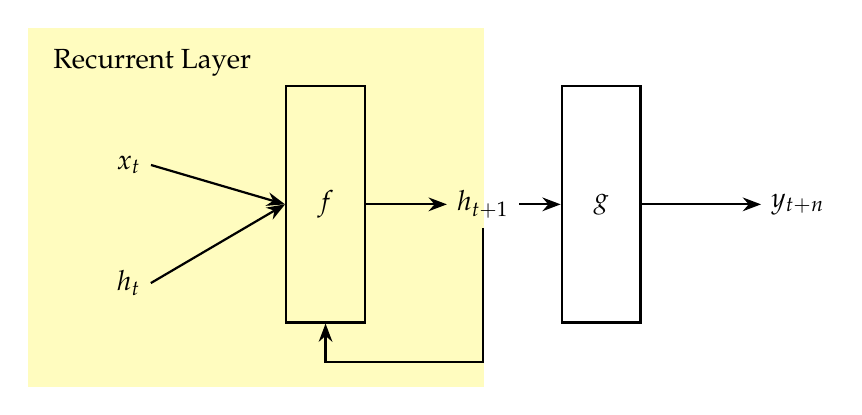
\begin{tikzpicture}[>=Stealth, thick, node distance=1.5cm]
      \tikzset{
      function/.style={rectangle, minimum width=1cm, minimum height=3cm, text centered, draw=black},
      signal/.style={circle, minimum size=0.5cm, text centered, draw=black},
      line/.style={draw, ->} % Define line style if needed
    }


    % Nodes
    \node (input) (input1) {\(x_t\)};
    \node (input) [below of=input1] (input2) {\(h_t\)};
    \node [function, right of=input1, xshift=1cm, , yshift=-0.5cm] (functionF) {\(f\)};
    \node [function, right of=functionF, xshift=2cm] (functionG) {\(g\)};
    \node (input)[right of=functionG, xshift=1cm] (output) {\(y_{t+n}\)};
    \node (input) [right of=functionF, xshift=0.5cm] (ht) {\(h_{t+1}\)};
    \node [above of=functionF, node distance=1.8cm, xshift=-2.2cm] (recurrentLabel) {Recurrent Layer};

    
    % Edges
    \draw[->] (input1.east) -- (functionF.west);
    \draw[->] (input2.east) -- (functionF.west);
   % \draw[->] (functionF.east) -- node[above] {\(h_{t+1}\)} (functionG.west);
    \draw[->] (functionG.east) -- (output.west);
    \draw[->] (functionF.east) -- (ht.west);
    \draw[->] (ht.east) -- (functionG.west);
    \draw[->] (ht) |- ++(0,-2) -| (functionF.south);
   
    % Background
    \begin{scope}[on background layer]
      \fill[yellow!25] ([shift={(-1,1.5)}]input1.north west) rectangle ([shift={(1.5,-0.8)}]functionF.south east);

    \end{scope}
     

    \end{tikzpicture}
  \end{adjustbox}
  \label{fig:RNN}
  \caption{Recurirsive Neural Network (RNN)}
\end{figure}

\begin{itemize}
  \item \( x_t \in \mathbb{R} \) denotes the input at time step \( t \). For simplicity, \( x_t \) is assumed to be a scalar with a single feature. This concept can be generalized to a \( d \)-dimensional feature vector.
  \item \( y_{t+1} \in \mathbb{R} \) represents the output of the network at time step \( t+1 \).
  \item \( h_t \in \mathbb{R}^m \) stores the values of the hidden units or states at time \( t \), also known as the current context.  
  \item \( h_{t+1} \in \mathbb{R}^m \) denotes the hidden state at time \( t+1 \)
\end{itemize}

At every time step, the network can be unfolded for \( k \) time steps to obtain the output at time step \( k + 1 \). This unfolded network is akin to a feedforward neural network.
The rectangle in the unfolded network indicates an operational sequence.
An example of single layer RNN is shown in the figure below:

\begin{figure}[ht]
  \centering
  \begin{adjustbox}{scale=0.9 } 
  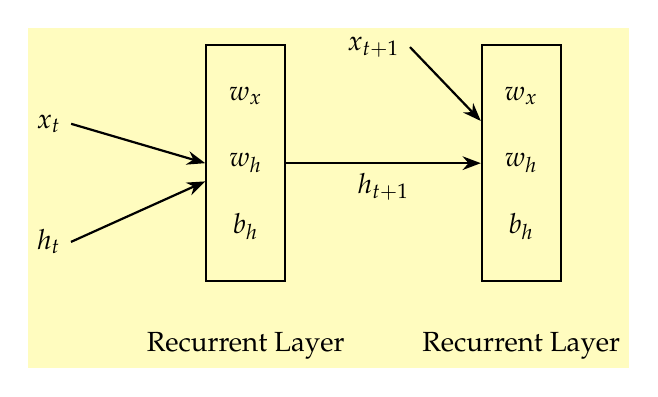
\begin{tikzpicture}[>=Stealth, thick, node distance=1.5cm]
      \tikzset{
      function/.style={rectangle, minimum width=1cm, minimum height=3cm, text centered, draw=black, align=center},
      signal/.style={circle, minimum size=0.5cm, text centered, draw=black},
      line/.style={draw, ->} % Define line style if needed
    }


    % Nodes
    \node (input) (input1) {\(x_t\)};
    \node (input) [below of=input1] (input2) {\(h_t\)};
    \node [function, right of=input1, xshift=1cm, , yshift=-0.5cm] (functionF) {\(w_x\)\\  \\ \(w_h\)\\ \\ \(b_h\)};
    \node [function, right of=functionF, xshift=2cm] (functionG) {\(w_x\) \\ \\ \(w_h\) \\ \\ \(b_h\)};
    \node (input) [above left = -0.3cm and 0.9cm of functionG, name=xt1] {\(x_{t+1}\)};

    \node [below = 0.5 of functionF, node distance=0.5cm]  (recurrentLabel) {Recurrent Layer};
    \node [below = 0.5 of functionG, node distance=0.5cm ] (recurrentLabel) {Recurrent Layer};



    
    % Edges
    \draw[->] (input1.east) -- node[midway, above] {} (functionF.west);
    \draw[->] (input2.east) -- node[midway, below] {}(functionF);
    
    \draw[->,] (functionF) -- (functionG) node [midway, below] {\(h_{t+1}\)} ;
    \draw[->] (xt1.east) -- (functionG);
   
    \begin{scope}[on background layer]
      \fill[yellow!25] (current bounding box.south west) rectangle (current bounding box.north east);
    \end{scope}
     

    \end{tikzpicture}
  \end{adjustbox}
  \label{fig:RNN_single_layer}
  \caption{Recurirsive Neural Network single layer}
\end{figure}

\begin{itemize}
  \item \( w_x \in \mathbb{R}^m \) are weights associated with inputs in the recurrent layer
  \item \( w_h \in \mathbb{R}^{m \times m} \) are weights associated with hidden units in the recurrent layer
  \item \( w_y \in \mathbb{R}^m \) are weights associated with hidden units to output units
  \item \( b_h \in \mathbb{R}^m \) is the bias associated with the recurrent layer
  \item \( b_y \in \mathbb{R} \) is the bias associated with the feedforward layer

\end{itemize}


For instance, with an activation function \( f \), the next hidden state is computed as:

\[ h_{t+1} = f(x_t, h_t, w_x, w_h, b_h) = f(w_x x_t + w_h h_t + b_h) \]

The output \( y_t \) at time \( t \) is determined by:

\[ y_t = f(h_t, w_y) = f(w_y \cdot h_t + b_y) \]

Here, \( \cdot \) signifies the dot product.\\
Consequently, during the feedforward pass of an RNN, the network computes the values of the hidden units and the output after \( k \) time steps. The network's weights are temporally shared. Each recurrent layer possesses two sets of weights: one for the input and another for the hidden units. The last feedforward layer, which calculates the final output for the \( k \)th time step, resembles a conventional layer in a traditional feedforward network.

\subparagraph{The Activation Function}

Any activation function may be employed within the recurrent neural network. Commonly used functions include:

\begin{itemize}
  \item Sigmoid function: \( \sigma(x) = \frac{1}{1 + e^{-x}} \)
  \item Tanh function: \( \tanh(x) = \frac{e^{2x} - 1}{e^{2x} + 1} \)
  \item ReLU function: \( \text{ReLU}(x) = \max(0, x) \)
\end{itemize}


\paragraph{Training and Vanishing Gradient}
Training neural networks involves adjusting their weights to minimize the difference between the predicted output and the actual target values.
For networks that process sequential data, like time series or natural language, this training must account for the temporal dependencies within the data.
Recurrent Neural Networks (RNNs) are specifically designed for this purpose, capable of maintaining state across sequential inputs through their looping architecture. 
However, training RNNs presents unique challenges due to their recurrent nature, necessitating specialized techniques to effectively learn from sequences. 

\begin{itemize}
\item \textbf{Unrolling the RNN Through Time :}

To apply BPTT, we first unroll the RNN across time, transforming it into an equivalent deep feedforward network. 
This unrolled structure maps each time step to a distinct layer in the network, facilitating the application of backpropagation as in traditional neural networks. 
The unrolled RNN can be mathematically represented as:

\begin{align*}
x_t & : \text{Input at time step } t, \\
h_t & = f(W_{hh}h_{t-1} + W_{xh}x_t + b_h) : \text{Hidden state at time step } t, \\
o_t & = g(W_{ho}h_t + b_o) : \text{Output at time step } t,
\end{align*}

where $f$ and $g$ denote non-linear activation functions, $W_{hh}$, $W_{xh}$, and $W_{ho}$ are weight matrices, and $b_h$, $b_o$ are bias vectors.

\item \textbf{Forward Pass :}

During the forward pass, we sequentially compute the activations and outputs for each time step, from $t=1$ to $T$, where $T$ is the sequence length. This process mirrors the execution of a feedforward neural network but incorporates temporal dependencies through the hidden states.

\item \textbf{Computing the Cost:}

Following the forward pass, the network's performance is evaluated using a cost function $C$, which measures the discrepancy between the predicted output sequence $\{o_1, o_2, ..., o_T\}$ and the target sequence. 
The choice of $C$ is dependent on the task, with Mean Squared Error (MSE) and Cross-Entropy being common choices for regression and classification tasks, respectively.

\item \textbf{Backward Pass (BPTT) :}

BPTT involves the backward propagation of the cost function's gradients through the unrolled network, extending traditional backpropagation to account for the network's temporal structure. 
The gradients of $C$ with respect to the weights, such as $\frac{\partial C}{\partial W_{hh}}$, $\frac{\partial C}{\partial W_{xh}}$, and $\frac{\partial C}{\partial W_{ho}}$, are computed using the chain rule and aggregated over all time steps, facilitating the update of weights based on their influence on future outputs.

\item \textbf{Weight Update :}

The final step in BPTT is updating the network's weights using the computed gradients. 
This is typically done using optimization algorithms like Stochastic Gradient Descent (SGD) or Adam, with update equations of the form:

\[
W = W - \eta \frac{\partial C}{\partial W},
\]

where $W$ represents the weight matrices ($W_{hh}$, $W_{xh}$, $W_{ho}$) and $\eta$ is the learning rate.


\end{itemize}


A significant challenge in the Backpropagation Through Time (BPTT) process is the phenomenon referred to as the \textit{vanishing gradient problem}. 
This issue predominantly arises in scenarios involving the processing of long time series data. As the gradient of the cost function with respect to the network's weights is propagated backward through time, its magnitude diminishes exponentially. 
This attenuation is a consequence of the repeated multiplication of gradients at each timestep, which are often less than one in magnitude. Consequently, this results in exceedingly small gradient values as one moves further back in time. The direct implication of this phenomenon is the negligible adjustment of weights corresponding to the earlier portions of the input sequence, thereby leading to slow convergence rates and a pronounced difficulty for the network in learning dependencies across extended sequences.

\paragraph{Vaniscing Gradient Problem}

The core of the issue comes from the characteristics of certain activation functions, notably the sigmoid function and the hyperbolic tangent function (\(\tanh\)). 
The sigmoid function, represented as \(\sigma(x)\), and the hyperbolic tangent function, denoted as \(\tanh(x)\), are mathematically articulated as follows:
\begin{align}
\sigma(x) &= \frac{1}{1 + e^{-x}}, \\
\tanh(x) &= \frac{e^{x} - e^{-x}}{e^{x} + e^{-x}}.
\end{align}

effectively squeezing an extensive range of input values into a narrow band between 0 and 1, for the sigmoid, and -1 to 1, for the tanh . 

This compression of input values means that large variations in input can result in disproportionately small changes in output. 
Consequently, the derivatives of these functions, crucial for the backpropagation algorithm, are significantly small in magnitude. 
For both functions, this effect is more pronounced for inputs of large magnitude, where the slope of the curve flattens out, leading to derivatives that approach zero.

\begin{figure}[ht]
  \centering
  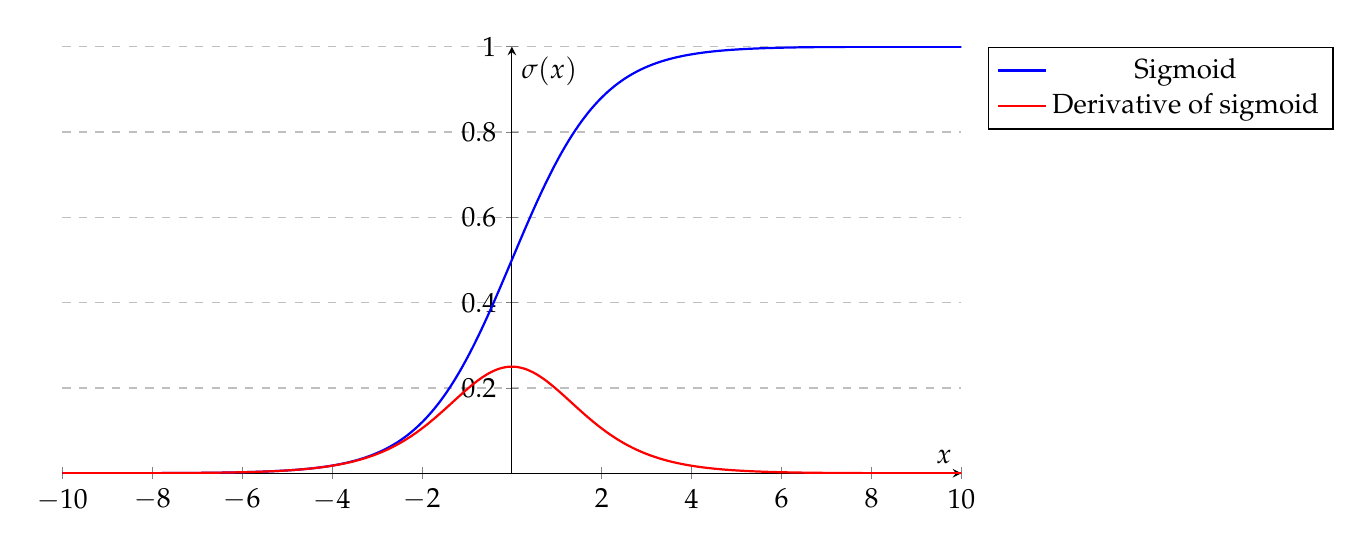
\begin{tikzpicture}
    \begin{axis}[
        axis lines=middle,
        xlabel={$x$},
        ylabel={$\sigma(x)$},
        xmin=-10, xmax=10,
        ymin=0, ymax=1,
        legend pos=outer north east,
        ymajorgrids=true,
        grid style=dashed,
        width=13cm, % Adjusted to your new width
        height=7cm, % Adjusted to your new height
    ]

    \addplot[
        color=blue,
        domain=-10:10,
        samples=100,
        smooth,
        thick,
    ]
    {1/(1+exp(-x))};
    \addlegendentry{Sigmoid}

    \addplot[
        color=red,
        domain=-10:10,
        samples=100,
        smooth,
        thick,
    ]
    {exp(x)/(1+exp(x))^2};
    \addlegendentry{Derivative of sigmoid}

    \end{axis}
  \end{tikzpicture}
  \caption{The sigmoid function and its derivative}
  \label{fig:Sigmoid}
\end{figure}

The sigmoid function is characterized by its distinctive S-shaped curve, serving as a pivotal nonlinear activation function in neural networks.\\
One of its notable features is the relationship between the input magnitude and the rate of change in the output. 
As the absolute value of the input escalates, the incremental change in the output significantly diminishes, leading to a derivative that approaches zero. 

Mathematically, the derivative of the sigmoid function, denoted as $\sigma'(x)$, can be expressed as:
\begin{equation}
\sigma'(x) = \sigma(x) \cdot (1 - \sigma(x)),
\end{equation}
where $\sigma(x)$ is the sigmoid function itself. 

In networks with a shallow architecture and fewer layers employing these activations, the vanishing gradient is less of an issue. 
However, the problem escalates with increased network depth, making the gradient too small for effective training.


\subsection{Long Short-Term Memory (LSTM) Networks}

LSTMs, as discussed by A. Graves et al.~\cite{graves2012long}, were designed to specifically address the challenges encountered with traditional RNNs, notably the vanishing gradient problem. 
Unlike standard RNNs, LSTMs incorporate a sophisticated gating mechanism to control the flow of information and gradients within the network.\\
This design significantly mitigates the vanishing gradient issue, enabling the network to learn from and remember information over extended sequences more effectively.
\newpage
The figure below illustrates the internal structure of an LSTM cell, showcasing its unique components:

\begin{figure}[ht]
  \centering
  \includegraphics[scale=0.2]{Figures/Chapter4/lstm_schematic_improved-transformed.png}
  \caption[LSTM Cell Structure]{LSTM Cell Structure}
  \label{fig:LSTM Cell Structure}
    
\end{figure}

LSTM cells include three critical gates: the input gate, the forget gate, and the output gate. 
These gates collectively manage the cell's memory, determining what information to retain, discard, and output. \\
This gating mechanism is pivotal for the LSTM's ability to modulate the gradient flow during backpropagation, directly addressing the vanishing gradient problem by maintaining gradient magnitude across long sequences.
The LSTM cell's core components are as follows:

\begin{itemize}

\item  \textbf{Forget Gate :}The forget gate plays a vital role in the LSTM architecture by deciding which information from the cell state should be kept or forgotten. It employs a sigmoid function to generate values between 0 and 1, with these values indicating the extent to which information is preserved or discarded.\\ 
This selective memory process enables LSTMs to focus on relevant information while minimizing unnecessary data retention, aiding in the preservation of gradient significance.

\item  \textbf{Input Gate and Output Gate :}The input gate is responsible for updating the cell state with new information. It operates in two steps: a sigmoid layer determines which values will be updated, and a tanh layer generates new candidate values.
 Conversely, the output gate decides what the next hidden state should be, which includes the filtered cell state information to be used in output.\\ 
 These gates ensure the network's ability to capture essential details for the task at hand, enhancing its long-term dependency modeling capabilities.

The operation of both the input and output gates ensures that if the outcome of these gates is close to 1, gradients can pass through without significant attenuation.Conversely, outcomes near 0 block the gradient flow. \\
This dynamic allows LSTMs to mitigate the vanishing gradient problem effectively.

\item  \textbf{Memory Cell State :}The memory cell state is the core component that allows LSTMs to retain information across time steps. It integrates inputs from the current time step and previous cell state, facilitating the network's ability to maintain a continuous flow of relevant information through the sequence. \\
The additive nature of the cell state updates helps to sustain gradient flow across long sequences, ensuring that LSTMs can capture and leverage long-range dependencies in the data.

\end{itemize}

\begin{itemize}
  \item \textbf{Forget Gate:} The forget gate plays a vital role in the LSTM architecture by deciding which information from the cell state should be kept or forgotten. It employs a sigmoid function to generate values between 0 and 1, with these values indicating the extent to which information is preserved or discarded.
  \[
  f_t = \sigma(W_f \cdot [h_{t-1}, x_t] + b_f)
  \]
  This selective memory process enables LSTMs to focus on relevant information while minimizing unnecessary data retention, aiding in the preservation of gradient significance.

  \item \textbf{Input Gate:} The input gate is responsible for updating the cell state with new information. It operates in two steps: a sigmoid layer determines which values will be updated, and a tanh layer generates new candidate values.
  \[
  i_t = \sigma(W_i \cdot [h_{t-1}, x_t] + b_i)
  \]
  \[
  \tilde{C}_t = \tanh(W_C \cdot [h_{t-1}, x_t] + b_C)
  \]
  Conversely, the output gate decides what the next hidden state should be, which includes the filtered cell state information to be used in output.

  \item \textbf{Cell State Update:} The memory cell state is the core component that allows LSTMs to retain information across time steps. It integrates inputs from the current time step and previous cell state, facilitating the network's ability to maintain a continuous flow of relevant information through the sequence.
  \[
  C_t = f_t \ast C_{t-1} + i_t \ast \tilde{C}_t
  \]
  The additive nature of the cell state updates helps to sustain gradient flow across long sequences, ensuring that LSTMs can capture and leverage long-range dependencies in the data.

  \item \textbf{Output Gate:} Determines the next hidden state, which includes the filtered cell state information to be used in outputs. The operation of the output gate ensures that gradients can pass through effectively, making it a key component in mitigating the vanishing gradient problem.
  \[
  o_t = \sigma(W_o \cdot [h_{t-1}, x_t] + b_o)
  \]
  \[
  h_t = o_t \ast \tanh(C_t)
  \]
\end{itemize}

\subsection{LSTM Intent Recognition Architecture}


 The application of theoretical approaches to intent recognition necessitates an investigation into various methodologies, with a particular focus on Long Short-Term Memory (LSTM) networks. 
 As detailed by Shao-Wen Wu et al.~\cite{wu2019predicting}, LSTM networks excel at understanding the complex patterns in data indicative of human intent. \\
 This research employs LSTM networks to estimate the parameters of a Beta distribution, demonstrating the networks' proficiency in accurately predicting human intentions, even in scenarios of incorrect teleoperation or obstacle avoidance, thus underscoring the model's dependability.

 Despite the effectiveness and reliability of this approach, it is not devoid of limitations. 
 A significant constraint is the assumption that objects remain stationary within their initial training environment. \\
 Any movement of these objects outside the direct view of the camera compromises the reliability of the alpha and beta parameters of the Beta distribution, leading to diminished accuracy in predictions.
 
In response to these impediments,in this thesis, the network will be assume the role of a binary classifier. 
This model, through the analysis of the end effector's distance and direction relative to an object, determines the likelihood of the object being the intended target for grasping. \\
Such an approach not only permits the LSTM to discern the complex dynamics between the input and output parameters, thereby enhancing its generalization capabilities, but also enables the adaptation of the model to accommodate the displacement of objects within the spatial domain without necessitating retraining.

Furthermore, the introduction of modularity into the model represents a significant advancement; by dedicating a distinct LSTM to each object, as show in figure ... the framework achieves scalability, allowing for its replication across multiple objects within a scene. \\
\begin{figure}[H]
  \centering
  
  \includegraphics[scale=0.5]{Figures/Chapter4/lstm_modularity.png}

  \caption{LSTM Model Modularity}
  \label{fig:LSTM Model Modularity}
\end{figure}




This characteristic ensures the model's viability in real-world scenarios, which are typified by the simultaneous presence of multiple objects, though it also necessitates an acknowledgment of the potential limitations posed by environmental clutter and computational resource constraints.

Central to this enhanced methodological approach is the objective of minimizing the model's inherent bias, thereby granting the LSTM the autonomy to independently identify and learn the subtle interrelations between distance and direction and their impact on object identification. 
This capacity for autonomous learning is imperative for the development of an intent recognition system that is not only efficient and adaptable but also robust enough to operate effectively within the complexities of real-world environments.\\
\newpage

Below a schematic of the LSTM model architecture is shown:

\begin{figure}[H]
  \centering
  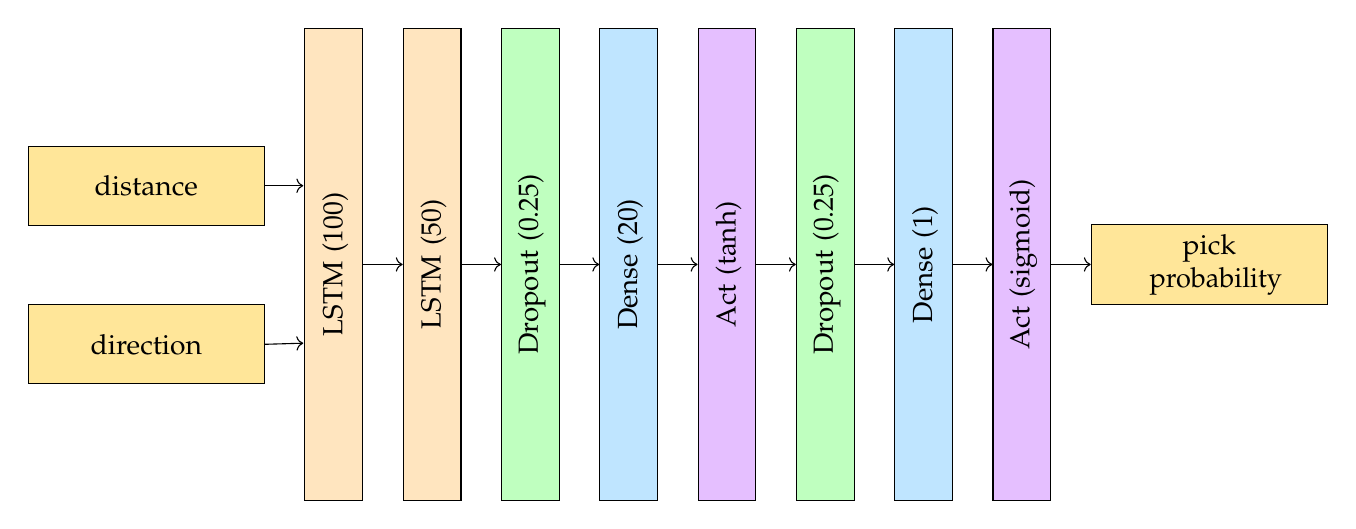
\begin{tikzpicture}[
    node distance=1 cm and 0.5 cm,
    block_inout/.style={
      rectangle,
      draw,
      fill=yellow25,
      text width=1.5cm,
      align=center,
      minimum height=1cm,
      minimum width=3cm
    },
    block_lstm/.style={
      rectangle,
      draw,
      fill=orange25,
      text width=0.5 cm,
      align=center,
      minimum height=6cm,
      minimum width=0.55cm,
    },
    block_dp/.style={
      rectangle,
      draw,
      fill=green25,
      text width=0.5cm,
      align=center,
      minimum height=6 cm,
      minimum width=0.55cm,
    },
    block_dens/.style={
      rectangle,
      draw,
      fill=blue25,
      text width=0.5cm,
      align=center,
      minimum height=6cm,
      minimum width=0.55cm,
    },
    block_act/.style={
      rectangle,
      draw,
      fill=purple25,
      text width=0.5cm,
      align=center,
      minimum height=6cm,
      minimum width=0.55cm,
    },
    line/.style={draw, ->} % Define line style if needed
  ]

  % Nodes
  \node [block_inout] (input1) {distance};
  \node [block_inout, below=of input1] (input2) {direction};

  \node (distanceinput) at (2,0) [inner sep=0,minimum size=0] {};
  \node (directioninput) at (2,-2) [inner sep=0,minimum size=0] {};
  \node (center) at (1.5,-1) [inner sep=0,minimum size=0] {};


  \node [block_lstm, right=of center ] (lstm) {\rotatebox{90}{LSTM (100)}};
  \node [block_lstm, right=of lstm] (lstm1) {\rotatebox{90}{LSTM (50)}};

  \node [block_dp, right=of lstm1] (dropout1) {\rotatebox{90}{Dropout (0.25)}};
  \node [block_dens, right=of dropout1] (dense1) {\rotatebox{90}{Dense (20)}};
  \node [block_act, right=of dense1] (activation1) {\rotatebox{90}{Act (tanh)}};
  
  \node [block_dp, right=of activation1] (dropout2) {\rotatebox{90}{Dropout (0.25)}};
  \node [block_dens, right=of dropout2] (dense2) {\rotatebox{90}{Dense (1)}};
  \node [block_act, right=of dense2] (activation2) {\rotatebox{90}{Act (sigmoid)}};

  \node [block_inout, right=of activation2] (output1) {pick\\ probability};
 

  % Arrows
  \draw[line] (input1.east) -- (distanceinput.west);
  \draw[line] (input2.east) -- (directioninput.west);
  \draw[line] (lstm) -- (lstm1);
  \draw[line] (lstm1) -- (dropout1);
  \draw[line] (dropout1) -- (dense1);
  \draw[line] (dense1) -- (activation1);
  
  \draw[line] (activation1) -- (dropout2);
  \draw[line] (dropout2) -- (dense2);
  \draw[line] (dense2) -- (activation2);
  \draw[line] (activation2) -- (output1);


\end{tikzpicture}
  \caption{LSTM Model Architecture}
  \label{fig:LSTM Model Architecture}
\end{figure}

To arrive a this final model, it was vital to carfelly plan evry step of the process, from the pre-processing of the data to modelling of each layer of the network.\\
since a minor change in the architecture of the network can lead to a significant change in the performance of the model, it was important to carefully plan each step of the process.\\

\paragraph{Pre-Processing of the Data}

The initial step in developing the model involved setting the number of neurons for the first LSTM layer. 
The LSTM, being a recurrent neural network, processes inputs sequentially through its repetitive cell structure. 
This means each cell within the layer handles a distinct input from the time sequence; specifically, as showcased in figure \label{RNN_single_layer}, the first cell processes the first input, the second cell the second input, and so on.

Selecting the appropriate number of cells in this layer is crucial. 
This choice is one of the first and most significant hyperparameters to be determined, directly impacting the model's capacity and computational demands.
Once this hyperparameter is established, it sets a foundational aspect of the model's architecture that is not easily modified later.

Analysis of data from 26 teleoperation experiments revealed an average of 2820 timesteps per experiment, with each experiment lasting around 26 seconds on average. 
Given this data, and to efficiently balance model complexity with the available computational resources, the neuron count for the first layer was set to 100. 

\paragraph{Stacked LSTM}

Recent studies on the application of Long Short-Term Memory (LSTM) networks to time series data, highlighted by \cite{cui2019deep} and \cite{9096332}, have revealed the efficacy of employing stacked LSTM layers in enhancing model performance. 
This design approach facilitates hidden layers in capturing progressively higher-level representations of the sequence data. 
Deep LSTM models, characterized by multiple LSTM hidden layers, create a structured flow where the output of one layer directly feeds into the subsequent layer, thereby significantly boosting the neural network's (NN) capability to learn. 

The hyperparameter configuration for modeling complex relationships was determined to be a two-layer LSTM structure. 
This choice was guided by the recognition that, although additional layers may enhance the model's ability to identify complex relationships among feature variables, a point is reached where further layers contribute to diminishing returns and increased risk of overfitting. Considering the dataset characterized by a relatively small number of input timesteps, incorporating a third layer would likely lead to overfitting, undermining the model's generalizability and efficiency.

\paragraph{Other layers}

To further mitigate the risk of overfitting in models with multiple layers, such as stacked LSTM networks, dropout layers have been introduced. 
This method involves randomly removing a specified proportion of neurons, as determined by the dropout ratio, from the network during each training iteration, effectively preventing their contributions to downstream neuron activation and halting weight updates during backpropagation for that iteration. For this experiment, the dropout ratio was set to 0.25, meaning 25\% of neurons in a layer are ignored at each training step, reducing the model's dependence on specific neurons and encouraging the learning of more robust features through forced feature redundancy. 
This approach not only helps in spreading out weights to diminish the likelihood of overfitting but also ensures the model does not rely too heavily on a small set of neurons, thereby improving its ability to generalize to unseen data. 
It is crucial to note that dropout is applied exclusively during training, with all neurons active during testing or evaluation phases, although their outputs are adjusted by the dropout rate to maintain consistency with the training environment

\begin{figure}[H]
  \centering
  
  \includegraphics[scale=0.4]{Figures/Chapter4/Droput.png}

  \caption{Effect of Dropout layer}
  \label{fig:Dropout}

\end{figure}

Another crucial part of the model, is th Fully-Connected layer, often referred to as a Dense layer in neural networks, which ensures complete interconnectivity between the neurons of consecutive layers. 
In such a layer, each neuron from the previous layer is linked to every neuron in the next, facilitating the layer's ability to derive a comprehensive linear combination of the input features. 
This configuration is instrumental in the network's capability to discern complex patterns within the depth of neural network models.\\
As seen in the stacked LSTM, which saw a reduction of cell from 100 to 50, the first Dense layer was configured to contain 20 neurons. 
This configuration aims to refine the feature space, enabling the network to concentrate on the most significant patterns identified by the LSTM layers, culminating in a final output layer comprising a single neuron. 
Both the LSTM and Dense layers employ the \textit{tanh} activation function.\\
The \textit{tanh} function is frequently chosen for LSTM layers due to its effectiveness in capturing complex patterns by introducing non-linearity into the network. 
Non-linearity is essential, as a purely linear model would be incapable of recognizing the intricate patterns present within the data.

Given the model's objective to classify the intention to pick or not pick an object based on the input, the task falls within the scope of a binary classification problem. 
Therefore, the architecture necessitates the inclusion of a Dense layer as the final component, distinguished by a single neuron utilizing a 'sigmoid' activation function. 
The 'sigmoid' function, characterized by its output range extending from 0 to 1, permits this concluding layer to map the features refined by antecedent layers into a predictive probability. 
This calculated probability serves to articulate the model's confidence in categorizing the input under one of two potential outcomes: the action to pick or the decision against picking the object.

\paragraph{Implementation of the model}
To deploy the LSTM model, it was done in python, more specifically using the keras library
Keras \cite{chollet2015keras} is a Python-based, open-source library designed to facilitate the development and training of deep learning models efficiently.
Acting as an interface for TensorFlow, it simplifies complex processes with predefined layers and algorithms for rapid experimentation. 
Emphasizing user-friendliness and modularity, Keras supports various backend engines, operates on both CPUs and GPUs, and enables quick prototyping with minimal code. 
This makes it accessible to users at all levels in the fields of machine learning and artificial intelligence.


'CODE?'





\subsection{Training the model}








 
\include{Chapters/Chapter5} 
\include{Chapters/Chapter6}
%\include{Chapters/ChapterExample}

%----------------------------------------------------------------------------------------
%	THESIS CONTENT - APPENDICES
%----------------------------------------------------------------------------------------

\appendix % Cue to tell LaTeX that the following "chapters" are Appendices

% Include the appendices of the thesis as separate files from the Appendices folder
% Uncomment the lines as you write the Appendices



\include{Appendices/AppendixA}
\include{Appendices/AppendixB}
%\include{Appendices/AppendixC}

%----------------------------------------------------------------------------------------
%	BIBLIOGRAPHY
%----------------------------------------------------------------------------------------
\medskip

\printbibliography[
    heading=bibintoc,
    title={Bibliography}
]

%----------------------------------------------------------------------------------------
%	ACKNOWLEDGEMENTS
%----------------------------------------------------------------------------------------

\include{Sections/Acknowledgements}

%----------------------------------------------------------------------------------------



%----------------------------------------------------------------------------------------
\end{document}  
